\documentclass[12pt]{article}
\usepackage{geometry}
\geometry{a4paper, margin=1in}
\usepackage{enumitem}
\usepackage{hyperref}
\usepackage{tocloft}
\usepackage{graphicx}
\hypersetup{
    colorlinks=true,
    linkcolor=blue,
    urlcolor=cyan,
}

\title{CS3338 Group 3 Design Specification\\\textbf{Want2Remember}}
\author{}
\date{}

\begin{document}

\maketitle
\thispagestyle{empty}
\newpage

\tableofcontents
\newpage

\section{Snapshot Objectives}

\subsection{Snapshot 1}
\textbf{Objective:} Our main objective is to develop a product that will support the performance of our user's short-term memory.capabilities.\newline
\textbf{Dependencies:}
\begin{itemize}
    \item JavaScript
    \item ReactJS
    \item GitHub
    \item JIRA and Agile Development Technology
    \item Firebase
\end{itemize}

\textbf{Delegation:} Initial feature to be completed: \textbf{Home Page}\newline
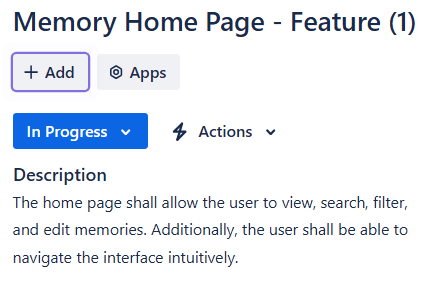
\includegraphics{snapshot1img1.png}\newline
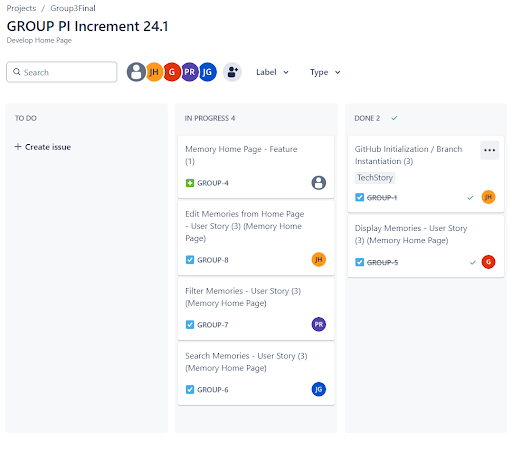
\includegraphics{snapshot1img2.png}
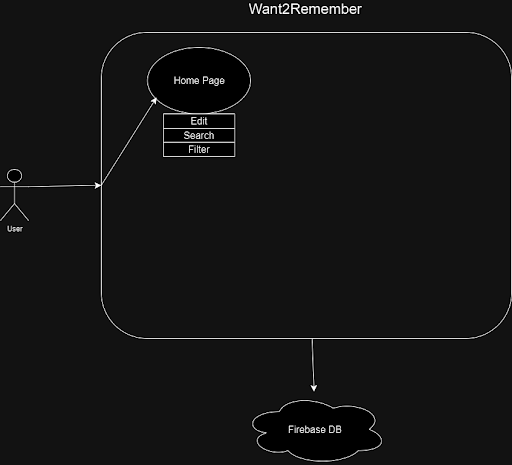
\includegraphics{snapshot1img3.png}
\textbf{Description:}The outer boundary represents the scope of the Want2Remember Product. Within shows different features as bubbles and their associated functionality as a table below. Outside of the boundary are external functionalities. The arrows represent the data flow of the product.


\subsection{Snapshot 2}
\textbf{Objective:} Develop and implement the Search/Filter functionality.\newline Dependencies Added :
\begin{itemize}
    \item
     TestRail
\end{itemize}
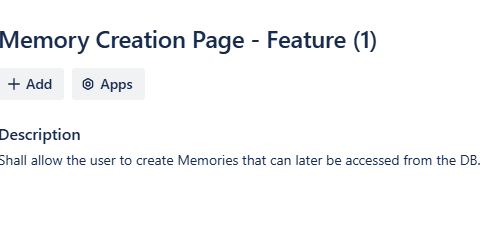
\includegraphics{snapshot2img1.png}
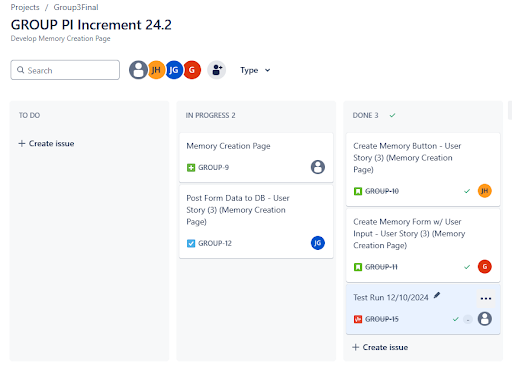
\includegraphics{snapshot2img2.png}
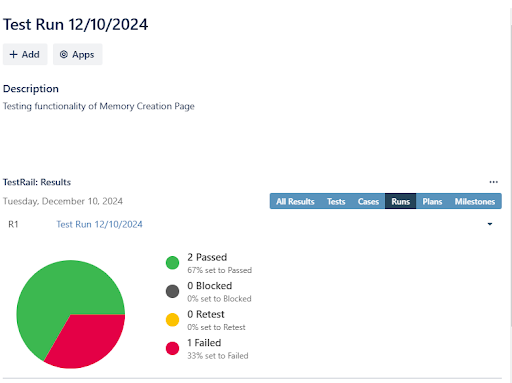
\includegraphics{snapshot2img3.png}
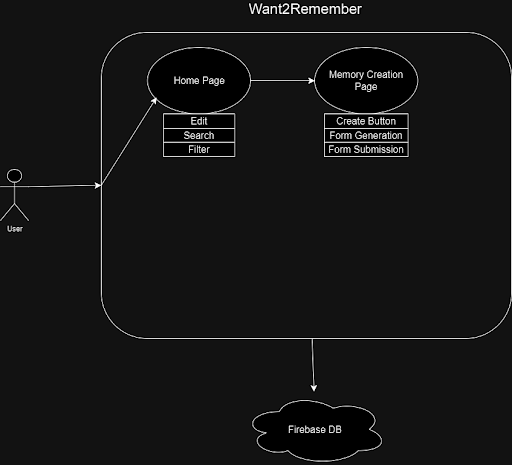
\includegraphics{snapshot2img4.png}

\subsection{Snapshot 3}
\textbf{Objective:} Complete and refine the Memory Creation Screen. 
\subsection{Snapshot 4}
\textbf{Objective:} Finalize the project.

\section{Design Breakdown}

\subsection{Home Page}
\begin{itemize}
    \item \textbf{Purpose:} Serve as the entry point for users. Provide navigation and a brief overview of the application's features.
    \item \textbf{Features:}
    \begin{itemize}
        \item Links to other pages (e.g., Memory Creation, Search/Filter).
        \item Firebase integration for user authentication.
    \end{itemize}
\end{itemize}

\subsection{Search/Filter Functionality}
\begin{itemize}
    \item \textbf{Purpose:} Enable users to efficiently search and filter their saved memories.
    \item \textbf{Features:}
    \begin{itemize}
        \item Search bar with dynamic filtering.
    \end{itemize}
\end{itemize}

\subsection{Memory Creation Screen}
\begin{itemize}
    \item \textbf{Purpose:} Provide a platform for users to create and save new memory entries.
    \item \textbf{Features:}
    \begin{itemize}
        \item Form for memory input (title, description, tags, etc.).
        \item Save button to store data in Firebase.
    \end{itemize}
\end{itemize}

\subsection{Firebase Integration}
\begin{itemize}
    \item \textbf{Purpose:} Serve as the backend service for authentication and data storage.
    \item \textbf{Features:}
    \begin{itemize}
        \item User authentication (login and registration).
        \item Real-time database for storing user-created memories.
    \end{itemize}
\end{itemize}

\section{Development Tools}
\begin{itemize}
    \item \textbf{JavaScript and ReactJS:} Used for front-end development.
    \item \textbf{GitHub:} Version control and collaboration.
    \item \textbf{JIRA:} Task tracking and Agile development.
    \item \textbf{Firebase:} Backend as a service for authentication and database management.
\end{itemize}
\section{Future Work}
\begin{itemize}
    \item \textbf{Improve Caregiver Features:} Some of the features that will help caregivers include GPS tracking of supported users and automatic role assignments. Another feature includes allowing the caregiver to remotely control the user’s app to showcase to the care receiver how to perform a specific task.
    \item \textbf{Medication Tracking:} Users will be able to set up reminders for medication and medication administration and save things like proofs of prescriptions.
    \item \textbf{Machine Learning/AI Features:} This can include using AI to improve interactivity with the app or implementing smart reminders that can further support people with cognitive impairments.
\end{itemize}

\end{document}


